\documentclass{article}
\usepackage{amsmath}
\usepackage{fullpage}
\usepackage{braket}
\usepackage{graphicx}
\begin{document}
\title{The VQE Energy Landscape}
\author{Harper Grimsley}
\maketitle
\section{Motivation}
Generalizability of the ADAPT-VQE ansatz to different Hamiltonians (e.g., $\hat{H}$ for the same molecule at different geometries) remains an open problem.  Unfortunately, it has proven challenging to recover a continuous potential energy surface for a "fixed" ADAPT ansatz subject to parameter re-optimization.  The underlying cause appears to be a failure of classical optimizers to identify the global energy minimum.
\section{Spurious Solutions}
Very large numbers of local minima apparently exist in the ADAPT-VQE ansatz, forming nearly continuous spectra in some cases:\\
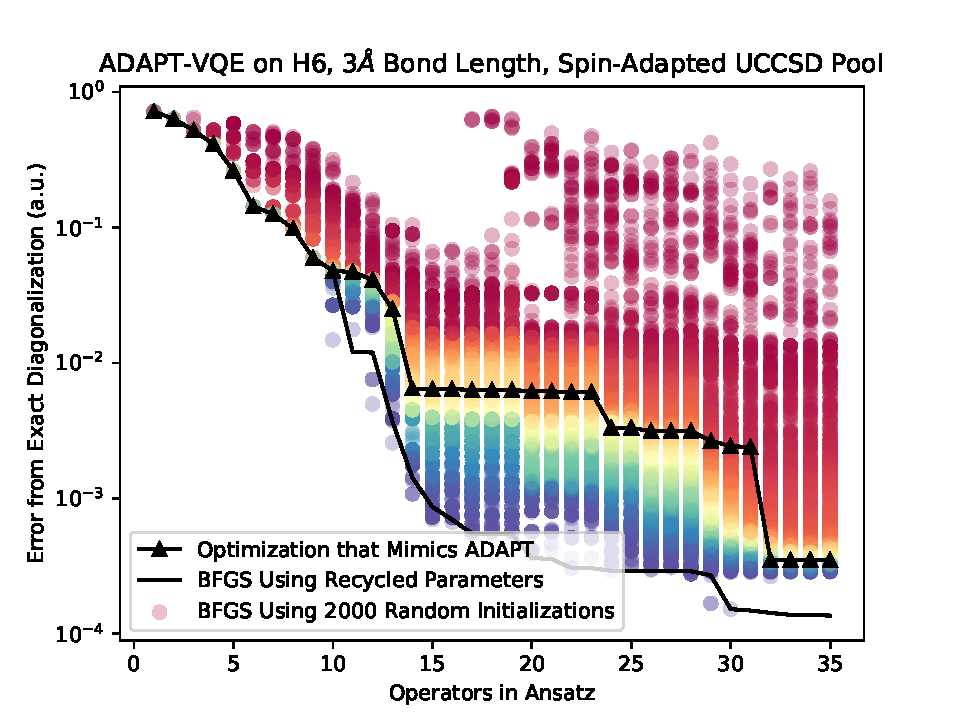
\includegraphics{big.pdf}\\
Note in particular that random guesses (each parameter is initialized randomly between -1 and 1) are occasionally better than a recycled ADAPT guess.  This occurrence appears to be unique to the Fermionic pool, or at least is so much more common that we only observe it in those pools.  (It occurs regardless of the use spin-adaptation, spin-complementation, or neither.)  By contrast, while many local minima are also seen in the Pauli pool, they are never better than the recycled guess.  
\section{Gimbal Locks}
Francesco Evangelista, Garnet Chan, and Gus Scuseria published a paper in 2019 on the expressibility of UCC-type ans{\"a}tze.  Notable points of the paper include:
\begin{itemize}
\item The UCCSD...N ansatz $\ket{\psi} = e^{\hat{T}-\hat{T}^\dagger}\ket{0}$ is able to exactly describe a CISD...N wavefunction $\ket{\Psi}$, assuming there are no pathological critical surfaces where the Jacobian of $\ket{\psi}$, $\hat{J}$ is rank-deficient.
\begin{equation}
\hat{J}_{ij} = \frac{\partial{\ket{\psi}_i}}{\partial t_j}
\end{equation}
\item Some (i.e., a non-empty set for any given $\ket{\Psi}$) 1st-order, Pseudo-Trotterized (No operators are repeated, but free control of the t-amplitudes is assumed) UCCSD...N ans{\"a}tze can express a CISD...N wavefunction $\ket{\Psi}$ unconditionally.
\item An infinite number of 1- and 2-particle, hole-particle generators can be used to approximate a pseudo-Trotterized UCCSD...N ansatz to arbitrary precision. That is, ignoring local minima and failures to add operators, ADAPT will eventually be exact when using the simple Fermionic pool. 
\end{itemize}
Jacobian analysis of $\ket{\Psi}$ without looking at the energy has proven interesting.  For example, the first time a recycled guess is worse than a random one is the 10th operator.  The solution ansatz's Jacobian obtained by initializing BFGS at the previous solution parameters, a very popular local minimum, has a distinctly small singular value, with the right-hand singular vector suggesting that the 1st and 10th parameter can be moved in opposite directions, with some minor relaxation between them, and the wavefunction will change very little.  This suggests the presence of a ``Gimbal lock,'' where the ansatz experiences an approximate loss of linear degrees of freedom. 
\section{Periodicity Issues with Symmetry-Adapted UCCSD}
Among the issues with global optimization of the Trotterized UCCSD landscape is the fact that symmetry-adapted Fermionic operators do not have the simple periodic structures possessed by, say, Pauli strings.  This makes it difficult to efficiently (or even fairly) sample the various amplitudes when doing things like choosing initial parameters for BFGS.  As an example, we consider the first two operators in the 3 \AA{} H$_6$ ansatz.  Some notational conventions will make this easier to follow:
\begin{align}
\hat{S}_{ij}^{ab} &= \frac{1}{2}\left(\hat{a}_{i\bar{j}}^{a\bar{b}}+\hat{a}_{j\bar{i}}^{a\bar{b}}+\hat{a}_{i\bar{j}}^{b\bar{a}}+\hat{a}_{j\bar{i}}^{b\bar{a}}\right)\\
\ket{S_{ij}^{ab}} &= \frac{1}{2}\left(\ket{\phi_{i\bar{j}}^{a\bar{b}}}+\ket{\phi_{j\bar{i}}^{a\bar{b}}}+\ket{\phi_{i\bar{j}}^{b\bar{a}}}+\ket{\phi_{j\bar{i}}^{b\bar{a}}}\right)\\
\ket{S_{k\bar{k}ij}^{c\bar{c}ab}} &= \frac{1}{2}\left(\ket{\phi_{k\bar{k}i\bar{j}}^{c\bar{c}a\bar{b}}}+\ket{\phi_{k\bar{k}j\bar{i}}^{c\bar{c}a\bar{b}}}+\ket{\phi_{k\bar{k}i\bar{j}}^{c\bar{c}b\bar{a}}}+\ket{\phi_{k\bar{k}j\bar{i}}^{c\bar{c}b\bar{a}}} \right)
\end{align}
The first operator acts on the reference as:
\begin{equation}
\ket{\psi_1} = e^{t_{02}^{35}\left(\hat{S}_{02}^{35}-\hat{S}_{35}^{02}\right)}\ket{0} = \cos^2\left(\frac{t_{02}^{35}}{\sqrt{2}}\right)\ket{0} + \frac{1}{\sqrt{2}}\sin\left(\sqrt{2}t_{02}^{35}\right)\ket{S_{02}^{35}} + \sin^2\left(\frac{t_{02}^{35}}{\sqrt{2}}\right)\ket{\phi_{0\bar{0}2\bar{2}}^{3\bar{3}5\bar{5}}}
\end{equation}
Every coefficient in $\ket{\psi_1}$ is periodic in $t_{02}^{35}$ with period $\sqrt{2}\pi$.  The second operator is where problems are introduced, however.  It can be shown that:
\begin{align}
\ket{\psi_2} &=  e^{t_{12}^{34}\left(\hat{S}_{12}^{34}-\hat{S}_{34}^{12}\right)}\ket{\psi_1} = \cos^2\left(\frac{t_{02}^{35}}{\sqrt{2}}\right)\left[\cos^2\left(\frac{t_{12}^{34}}{\sqrt{2}}\right)\ket{0} + \frac{1}{\sqrt{2}}\sin\left(\sqrt{2}t_{12}^{34}\right)\ket{S_{12}^{34}} + \sin^2\left(\frac{t_{12}^{34}}{\sqrt{2}}\right)\ket{\phi_{1\bar{1}2\bar{2}}^{3\bar{3}4\bar{4}}}\right]\\
&+\sin^2\left(\frac{t_{02}^{35}}{\sqrt{2}}\right)\ket{\phi_{0\bar{0}2\bar{2}}^{3\bar{3}5\bar{5}}}+\frac{1}{\sqrt{2}}\sin\left(\sqrt{2}t_{02}^{35}\right)\left[\cos\left(\frac{t_{12}^{34}}{2}\right)\ket{S_{02}^{35}}+\sin\left(\frac{t_{12}^{34}}{2}\right)\ket{S_{2\bar{2}01}^{3\bar{3}45}}\right]
\end{align}
Each coefficient in the above expansion is periodic (or constant) in $t_{12}^{34}$.  However, the coefficients in the first bracket have period $\sqrt{2}\pi$, while those in the second bracket have period $4\pi$.  These periods are \textit{incommensurable}- they have no least common multiple, so that there is no overall $t_{12}^{34}$ period of $\ket{\psi_2}$.  This lack of periodicity extends to the energy functional:  
\begin{align}
E_c[t_{12}^{34},t_{02}^{35}] &= \frac{1}{2}\cos^4\left(\frac{t_{02}^{35}}{\sqrt{2}}\right)\sin^2\left(\sqrt{2}t_{12}^{34}\right)\braket{S_{12}^{34}|\hat{H}_N|S_{12}^{34}} \\
&+\cos^4\left(\frac{t_{02}^{35}}{\sqrt{2}}\right)\sin^4\left(\frac{t_{12}^{34}}{\sqrt{2}}\right)\braket{\phi_{1\bar{1}2\bar{2}}^{3\bar{3}4\bar{4}}|\hat{H}_N|\phi_{1\bar{1}2\bar{2}}^{3\bar{3}4\bar{4}}}\\
&+\sin^4\left(\frac{t_{02}^{35}}{\sqrt{2}}\right)\braket{\phi_{0\bar{0}2\bar{2}}^{3\bar{3}5\bar{5}}|\hat{H}_N|\phi_{0\bar{0}2\bar{2}}^{3\bar{3}5\bar{5}}}\\
&+\frac{1}{2}\sin^2\left(\sqrt{2}t_{02}^{35}\right)\cos^2\left(\frac{t_{12}^{34}}{2}\right)\braket{S_{02}^{35}|\hat{H}_N|S_{02}^{35}}\\
&+\frac{1}{2}\sin^2\left(\sqrt{2}t_{02}^{35}\right)\sin^2\left(\frac{t_{12}^{34}}{2}\right)\braket{S_{2\bar{2}01}^{3\bar{3}45}|\hat{H}_N|S_{2\bar{2}01}^{3\bar{3}45}}\\
&+\cos^2\left(\frac{t_{02}^{35}}{\sqrt{2}}\right)\sin\left(\sqrt{2}t_{12}^{34}\right)\braket{0|\hat{H}_N|S_{12}^{34}}\\
&+\sqrt{2}\cos^2\left(\frac{t_{02}^{35}}{\sqrt{2}}\right)\sin\left(\sqrt{2}t_{02}^{35}\right)\cos\left(\sqrt{2}t_{12}^{34}\right)\braket{0|\hat{H}_N|S_{02}^{35}}\\
&+\sqrt{2}\cos^4\left(\frac{t_{02}^{35}}{\sqrt{2}}\right)\sin\left(\sqrt{2}t_{12}^{34}\right)\sin^2\left(\frac{t_{12}^{34}}{\sqrt{2}}\right)\braket{S_{12}^{34}|\hat{H}_N|\phi_{1\bar{1}2\bar{2}}^{3\bar{3}4\bar{4}}}\\
&+\cos^2\left(\frac{t_{02}^{35}}{\sqrt{2}}\right)\sin\left(\sqrt{2}t_{02}^{35}\right)\sin\left(\sqrt{2}t_{12}^{34}\right)\cos\left(\sqrt{2}t_{12}^{34}\right)\braket{S_{12}^{34}|\hat{H}_N|S_{02}^{35}}\\
&+\cos^2\left(\frac{t_{02}^{35}}{\sqrt{2}}\right)\sin\left(\sqrt{2}t_{02}^{35}\right)\sin\left(\sqrt{2}t_{12}^{34}\right)\sin\left(\frac{t_{12}^{34}}{2}\right)\braket{S_{12}^{34}|\hat{H}_N|S_{2\bar{2}01}^{3\bar{3}45}}\\
&+\sqrt{2}\cos^2\left(\frac{t_{02}^{35}}{\sqrt{2}}\right)\sin\left(\sqrt{2}t_{02}^{35}\right)\sin^2\left(\frac{t_{12}^{34}}{\sqrt{2}}\right)\sin\left(\frac{t_{12}^{34}}{2}\right)\braket{\phi_{1\bar{1}2\bar{2}}^{3\bar{3}4\bar{4}}|\hat{H}_N|S_{2\bar{2}01}^{3\bar{3}45}}\\
&+\sqrt{2}\sin^2\left(\frac{t_{02}^{35}}{\sqrt{2}}\right)\sin\left(\sqrt{2}t_{02}^{35}\right)\cos\left(\frac{t_{12}^{34}}{\sqrt{2}}\right)\braket{\phi_{0\bar{0}2\bar{2}}^{3\bar{3}5\bar{5}}|\hat{H}_N|S_{02}^{35}}\\
&+\sqrt{2}\sin^2\left(\frac{t_{02}^{35}}{\sqrt{2}}\right)\sin\left(\sqrt{2}t_{02}^{35}\right)\sin\left(\frac{t_{12}^{34}}{2}\right)\braket{\phi_{0\bar{0}2\bar{2}}^{3\bar{3}5\bar{5}}|\hat{H}_N|S_{2\bar{2}01}^{3\bar{3}45}}\\
&+\sin^2\left(\sqrt{2}t_{02}^{35}\right)\cos\left(\frac{t_{12}^{34}}{2}\right)\sin\left(\frac{t_{12}^{34}}{2}\right)\braket{S_{02}^{35}|\hat{H}_N|S_{2\bar{2}01}^{3\bar{3}45}}
\end{align}
For example, the first term has $t_{12}^{34}$ periodic in $\frac{\pi}{\sqrt{2}}$, while the fourth term has it periodic in $\frac{\pi}{2}$.  Thus, the energy cannot have an overall periodicity in $t_{12}^{34}$.  The energy landscape for this problem is pictured below for a relatively small region.\\
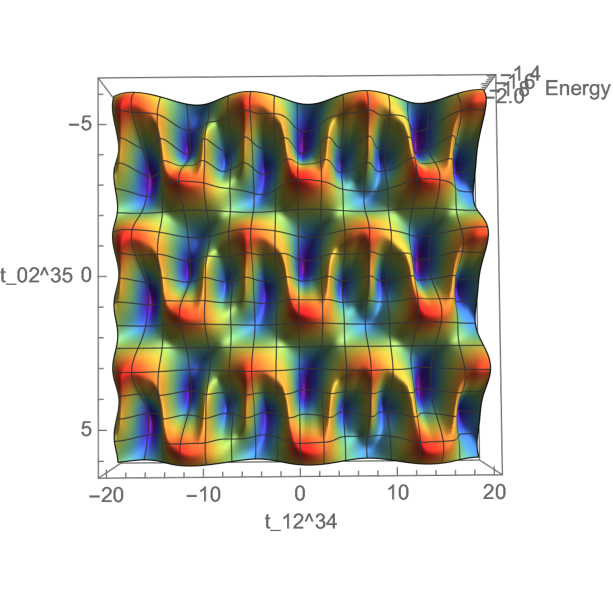
\includegraphics{non-periodic.pdf}\\
Below is a plot over a much larger range of $t_{12}^{34}$ values and a smaller range of $t_{02}^{35}$ values.  The grey plane at the top is the nearest minimum to the HF reference in the previous figure.  The energies are given relative to TRUCC, described in the next section.  The main takeaway is that if one assumes approximate periodicity in $t_{12}^{34}$, and doesn't sample it over the entire set of real numbers, they will not even get within chemical accuracy of the ansatz's full potential.\\
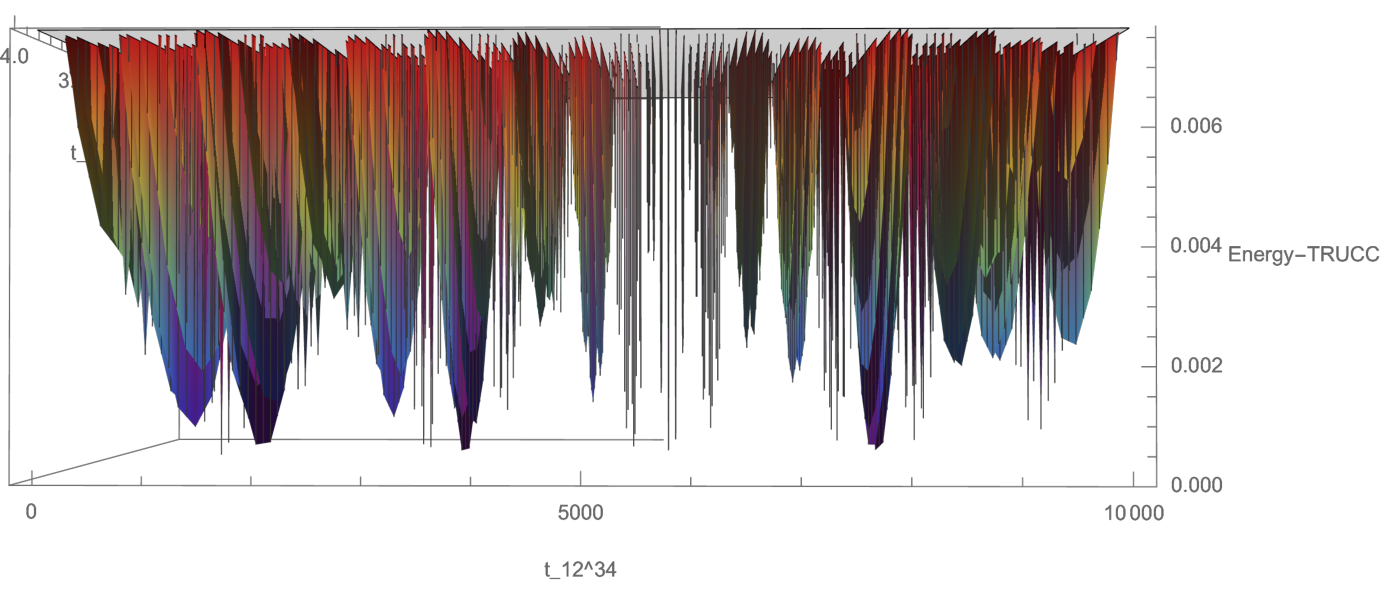
\includegraphics[width=\textwidth]{non-periodic_2.pdf}  

\subsection*{Conjecture About Periodicity Prediction}
Let $\hat{A}$ be an anti-Hermitian operator.  The action of $e^{\hat{A}t}\ket{\psi}$ (not necessarily normalized), has a fundamental, simple period in t of $\frac{2\pi}{\sqrt{-\lambda}}$ if and only if:
\begin{enumerate}
\item $\hat{A}\ket{\psi}\neq 0$
\item $\hat{A}\ket{\psi}$ is an eigenvector of $\hat{A}^2$ with eigenvalue $\lambda$. 
\end{enumerate}
By a simple period, we mean that there are not multiple terms with unique commensurable periods.  That is, two different periods with a least common multiple still aren't allowed.  E.g., $\sin(2t)+\sin(4t)$ is not simple by our criterion.  Note that if $\hat{A}^2 = -\hat{\mathbf{1}}$, as with the Pauli strings, $e^{\hat{A}t}$ is immediately made periodic in $2\pi$, regardless of what it is acting on.  I believe this conjecture can be used to show that the spin-complemented UCCSD pool should be periodic, at least for an $S_z$-pure reference. 
 
\subsection*{Conjecture Regarding A Fix to The Problem}
Let f(x) and g(x) be incommensurable, periodic functions of x with periods $T_f$ and $T_g$.  For any $\epsilon>0$, $y\in \mathbf{R}$, there exists an integer N such that $|g(x+NT_f)-g(y)|<\epsilon$.  If this is the case, it follows that in floating point arithmetic, the range of the objective functional $\mathcal{L}\left[f(x),g(x)\right]$ is equivalent to that of $\mathcal{L}\left[f(x),g(y)\right]$, and the arguments of $f$ and $g$ can be treated as two independent parameters, each of which is periodic, giving overall bounds on the optimization and avoiding artificial dependencies between $f$ and $g$.  (This approximation can be made whether or not the conjecture is true, and the variational principle still holds.)  I am tentatively calling it ``Topologically Relaxed UCC,'' or TRUCC.  I can rigorously show that the range of the TRUCC wavefunction in a bounded region is equivalent to the global range of UCC for a specific two-operator problem, and I don't think a general proof would be all that hard.\\
\par
My prescription would be to factorize each generator $\hat{A}$ by sorting all product states into minimal groups which are closed under the action of powers of $\hat{A}$, ignoring non-zero scalars.  For example, if $\hat{A} = \hat{a}_i^a +\hat{a}_{\bar{i}}^{\bar{a}}-\text{H.C.}$, the the group containing $\ket{0}$ would be 
\begin{equation}
\mathcal{G}_{i,\ket{0}} = \{\ket{0},\ket{\phi_i^a}+\ket{\phi_{\bar{i}}^{\bar{a}}},\ket{\phi_{i\bar{i}}^{a\bar{a}}}\} 
\end{equation}
The period of $\hat{A}_i$ should be constant for any starting guess in $\mathcal{G}_{i,{\ket{0}}}$, so that if $\mathcal{P}$ is the projector onto $\mathcal{G}_{i,{\ket{0}}}$, then $e^{\mathcal{P}\hat{A}_i\mathcal{P}\theta_i}$ is periodic in $\theta_i$ regardless of its target, with a well-defined period that can be classically determined.  Many of the minimal groups for a fermionic generator will have cardinality 1, since only $\hat{A}^0=\mathbf{I}$ does not destroy them.  (For Pauli strings, the groups would all have cardinality 2 due to the involutory nature of the operators.)  If we construct a whole set of projectors $\mathcal{P}_j$ this way:
\begin{align}
e^{\theta_i\hat{A}_i} &= e^{\theta_i\sum_j \mathcal{P}_j\hat{A}_i\mathcal{P}_j}\\
&= e^{\theta_i\sum_j \mathcal{P}_j\hat{A}_i\mathcal{P}_j}e^{\theta_i\sum_k \mathcal{P}_k\hat{A}_i\mathcal{P}_k}\dots
\end{align}
If we do this type of partitioning so that each of the new $e^{\theta_i\sum_j\mathcal{P}_j\hat{A}_i\mathcal{P}_j}$ rotations are mutually incommensurable in $\theta_i$, then, if I'm right, each rotation can have an independent parameter.  By adding the auxiliary parameters, we now have a product of periodic rotations, rather than one non-periodic rotation.  I believe these are the same.  If not, this is still a unitary rotation, so it won't break the variational principle.  We could simply replace the operator $\hat{A}_i$ with the generators it would get broken into when we construct the pool.  There are a limited number of group structures to compute for a given operator pool.   Alternatively, we only actually need the groups generated by non-zero powers of $\hat{A}$ on target states at any given time.  I am personally partial to the former choice, since I can theoretically just work out the topologically relaxed operators for six types of excitations, and then ADAPT's operator addition criterion won't unphysically think of separately parameterized rotations as being dependent when it's deciding whether to add them.    
\end{document}
